\documentclass{report}
\usepackage{graphicx}
\graphicspath{ {./screenshots/} }
\usepackage{titlesec}
\usepackage{amsmath}
\usepackage{amssymb}

\titleformat{\chapter}[display]
  {\normalfont\bfseries}{}{0pt}{\Large}
\titlespacing*{\chapter}{0pt}{-100pt}{25pt}


\begin{document}

\begin{center}
    \large Zusammenfassung
\end{center}

\begin{center}
    \Large \textit{Maschinelles Lernen}\\
    \vspace*{.5em}
    \normalsize \textit{WS 19/20}\\
    \vspace*{45em}
    \large \today
\end{center}

\newpage

\chapter{Mathematische Grundlagen}
\vspace*{-1.25em}
\section{Lineare Algebra}
\subsection{Skalarprodukt}
- Vektoren $x, y \in \mathbb{R}^n$: $x\circ y = \sum_{i=1}^n x_i\cdot y_i = x^Ty$\\
- $\begin{bmatrix}1\\2\end{bmatrix}\circ \begin{bmatrix}3\\4\end{bmatrix} = 1\cdot 3 + 2\cdot 4 = 11$
\subsection{Vektornorm}
$f: \mathbb{R}^n\rightarrow \mathbb{R}$ mit\\
\vspace*{-1.5em}
\begin{itemize}
  \item $f(x) = 0 \Rightarrow x = 0$
  \item $f(x + y) \leq f(x) + f(y)$ (\textit{Dreiecksgleichung})
  \item $f(\alpha x) = |\alpha|f(x)$
\end{itemize}
- $L_1$-Norm: $||x||_1 = \sum_i|x_i|$\\
- $L_2$-Norm: $||x||_2 = \sqrt{\sum_i x_i^2}$ (\textit{euklidische Norm})
\subsection{Matrizen}
- \textit{m} Zeilen und \textit{n Spalten}
A = $\begin{bmatrix}A_{11} & ... & A_{1n}\\A_{m1} & ... & A_{mn} \end{bmatrix}$,
$\begin{bmatrix}1 & 2\\3 & 4\\5 & 6\end{bmatrix}^T = \begin{bmatrix}1 & 3 & 5\\2 & 4 & 6\end{bmatrix}$\\
- $\begin{bmatrix}a & b & c\\d & e & f\end{bmatrix}\cdot \begin{bmatrix}g & h\\i & j\\k & l\end{bmatrix}$
= $\begin{bmatrix}ag + bi + ck & ah + bj + cl\\dg + ei + fk & dh + ej + fl\end{bmatrix}$,
$I = \begin{bmatrix}1 & 0 & 0\\0 & 1 & 0\\0 & 0 &1\end{bmatrix}$\\
- $A^{-1}A = I$ (Matrizen mit linear abhängigen Zeilen oder Spalten (niedriger Rang) sind nicht invertierbar)
\subsection{Hyperebene}
- x $\in$ $\mathbb{R}^d$ erfüllen Gleichung $w_0 + w_1x_1 + w2_x2 + ... + w_dx_d = 0$ ($w_0 + w^Tx = 0$)\\
- $d = 1$: Skalar ($w_0 + w_1x_1$), $d = 2$: Gerade ($w_0 + w_1x_1 + w_2x_2$), $d = 3$: Ebene\\
- Für einen Punkt $x$ entscheidet das Vorzeichen $sgn(w_0 + w^Tx)\in \{-1, 0, 1\}$ auf welcher Seite der Hyperebene er liegt (bzw. ob er auf ihr liegt)\\
\begin{center}
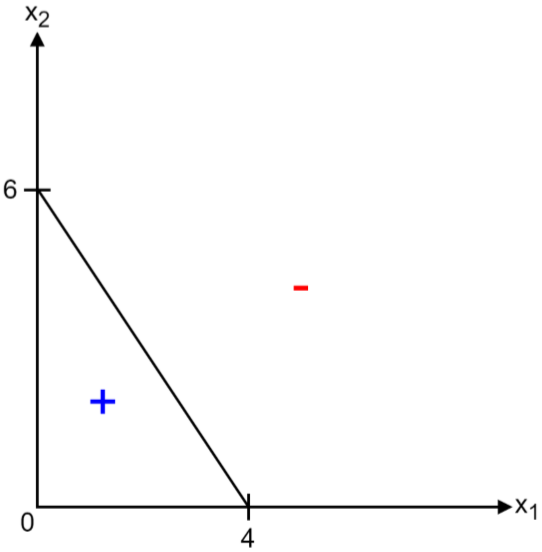
\includegraphics[scale=.2]{ml01_1} $1 - \frac{1}{4}x_1 - \frac{1}{6}x_2 = 0$
\end{center}

\section{Analysis}
\subsection{Kettenregel}
- Wenn $z$ von $y$ und $y$ von $x$ abhängt, dann gilt: $\frac{dz}{dx} = \frac{dz}{dy}\frac{dy}{dx}$\\
- $f(x) = g(h(x)) = \frac{1}{2}\cdot(x_1 - x_2)^2$ $\rightarrow$ $g(x) = \frac{1}{2}x^2$ und $h(x) = x_1 - x_2$\\
- $\frac{df}{dx_2} = \frac{dg}{dh}\frac{dh}{d_x2} = h(x)(-1) = -(x_1 - x_2) = x_2 - x_1$
\subsection{Partielle Ableitung}
$f(x) = 2x_1^3 - 5x_2^2 + 3$, $\frac{df}{dx_1} = 6x_1^2$, $\frac{df}{dx_2} = -10x_2$
\subsection{Gradient}
$\nabla f = \begin{bmatrix}\frac{df}{dx_1}\\ . \\. \\.\\\frac{df}{dx_n}\end{bmatrix}$, $f(x) = 2x_1^3 - 5x_2^2 + 3, \nabla f = \begin{bmatrix}6x_1^2\\-10x_2\end{bmatrix}$

\section{Was ist maschinelles Lernen}
\subsection{Paradigmenwechsel}
Es ist schwierig, den entsprechenden Programmcode manuell zu schreiben, daher wird ein anderes Paradigma verwendet:
\begin{center}
  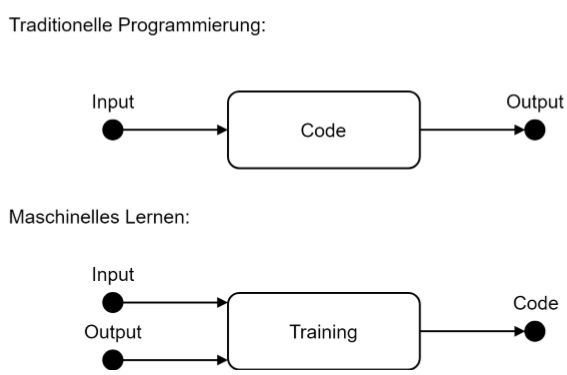
\includegraphics[scale=.4]{ml01_2}
\end{center}
Drei verschiedene Lernmethoden
\begin{itemize}
  \item Überwachtes Lernen (\textit{Supervised Learning})
  \item Unüberwachtes Lernen (\textit{Unsupervised Learning})
  \item Bestärkendes Lernen (\textit{Reinforcement Learning})
\end{itemize}

\subsection{Überwachtes Lernen}
- Ziel: finden einer Funktion $f: X \rightarrow Y$ wobei $X$ auch \textit{Features} und $Y$ auch \textit{Responses} genannt werden\\
- Eine perfekte Abbildung ist nicht möglich, es treten \textit{reduzierbare} Fehler (z.B. durch eine bessere Funktion $f$) und \textit{nicht reduzierbare} Fehler auf (z.B. Messfehler in Eingabedaten)

\end{document}